\documentclass[12pt,letterpaper]{article}
\usepackage{natbib}

%Packages
% \usepackage{textcomp}
% \usepackage{latexsym}
% \usepackage{url}
% \usepackage{amssymb}
% \usepackage{amsmath}
% \usepackage{mathtools}
% \usepackage{bm}
% \usepackage{array}
% \usepackage[version=3]{mhchem}
% \usepackage{ifthen}
% \usepackage{amsthm}
% \usepackage{amstext}
% \usepackage{enumerate}
% \usepackage{dcolumn}


\usepackage{epsfig}
\usepackage{graphicx}
\usepackage{caption}
\usepackage{hyperref}
\usepackage{lineno}
\usepackage{pdflscape}
\usepackage{mathtools}
\usepackage[osf]{mathpazo}
\usepackage{fullpage}
\usepackage{float}
\usepackage{xr} %linking to supplementaries
\externaldocument{supplementaries}

\pagenumbering{arabic}

%---------------------------------------------
%
%       START
%
%---------------------------------------------

\begin{document}
%Running head
\begin{flushright}
Version dated: \today
\end{flushright}

\bigskip
\begin{center}

\noindent{\Large \bf The what, how and why of trait-based analyses in ecology}
\bigskip

\noindent RH: The what, how and why of trait-based analyses

% \noindent {\normalsize \sc
% Thomas Guillerme$^{1,*}$, 
% Pedro Cardoso$^{2,3}$, %pedro.cardoso@helsinki.fi
% % Carlos P. Carmona$^{4}$,
% Maria Wagner J\o rgensen$^{4}$, %mwj207@student.bham.ac.uk
% Stefano Mammola$^{3,5,6}$, %stefanomammola@gmail.com
% Thomas J. Matthews$^{4,7}$}\\ % txm676@gmail.com
% \noindent {\small \it 
% $^1$School of Biosciences, The University of Sheffield, Sheffield, S10 2TN, United Kingdom.\\
% $^2$CE3C—Centre for Ecology, Evolution and Environmental Changes, CHANGE – Global Change and Sustainability Institute, Faculty of Sciences, University of Lisbon, Lisbon, Portugal\\
% $^3$Laboratory for Integrative Biodiversity Research (LIBRe), Finnish Museum of Natural History (Luomus), University of Helsinki, Helsinki, Finland\\
% % $^4$Institute of Ecology and Earth Sciences, University of Tartu, Tartu, Estonia\\
% $^4$School of Geography, Earth and Environmental Sciences and Birmingham Institute of Forest Research, University of Birmingham, Birmingham B15 2TT, UK\\
% $^5$Molecular Ecology Group (MEG), Water Research Institute, National Research Council (CNR-IRSA), Verbania Pallanza, Italy\\
% $^6$National Biodiversity Future Center, Piazza Marina 61, 90133 Palermo, Italy\\
% $^7$Centre for Ecology, Evolution and Environmental Changes/Azorean Biodiversity Group / CHANGE – Global Change and Sustainability Institute and Universidade dos Açores – Faculty of Agricultural Sciences and Environment; PT-9700-042, Angra do Hero\'ismo, A\c ores, Portugal.\\}

\end{center}
% \bigskip
% \noindent{*\bf Corresponding author.} \textit{t.guillerme@sheffield.ac.uk}\\ 

% \noindent (Keywords: Functional diversity, dissimilarity, disparity, patterns, processes, mechanisms)\\

% \begin{itemize}
%    \item Article type: Perspective
%    \item Number of words in the abstract: 189
%    \item Number of words in the main text: 3960
%    \item Number of words in the text box: 419
%    \item Number of references: 54
%    \item 3 Figures, 2 tables and 1 text box
% \end{itemize}

% \subsection{Statement of authorship}

% TG, PC, MWJ, SM and TJM designed the study, analysed the data and wrote the manuscript. TG wrote the code to analyse the data.

% \subsection{Data accessibility statement}

% All code and data required to reproduce this analysis is available on GitHub: \url{https://github.com/TGuillerme/eco_metrics_simulations/}.

% %---------------------------------------------
% %
% %       ABSTRACT
% %
% %---------------------------------------------

\newpage
%Line numbering
\modulolinenumbers[1]
\linenumbers

\section{Abstract}

Functional diversity is increasingly used alongside taxonomic diversity to describe populations and communities in ecology.
Indeed, functional diversity metrics allow researchers to summarise complex occupancy patterns in space and/or time across communities and/or populations in response to various stressors.
In other words, investigating what, how and why something is changing in an ecosystem by looking at changes of patterns under a certain process through a specific mechanism.
However, as the diversity of functional diversity metrics and methods increases, it is often not directly clear which metric is more readily appropriate for which question.
We studied the ability of different functional diversity metrics to recover patterns and signals from different processes linked to common assembly mechanisms in community ecology; such as environmental filtering, competitive exclusion, equalising fitness, and facilitation.
Using both simulated data and an empirical dataset affected by more complex and nuanced mechanisms, we tested the effectiveness of different space occupancy metrics to recover the simulated or empirical changes.
We show that different metrics perform differently when trying to capture signal from different approximation of common mechanisms relative to no mechanism at all (null).
For example competition was harder to disentangle from the null mechanisms compared to facilitation in our simulations.
This emphasises the importance of not using a one-size-fits-all metric.
Instead, researchers should carefully consider and test whether a particular metric will be effective in capturing a pattern of interest.

\noindent (Keywords: Functional diversity, dissimilarity, disparity, patterns, processes, mechanisms)\\

\newpage

\section{Introduction}

In the last two decades, there has been a progressive expansion in ecology and evolution studies from taxonomic-oriented approaches, with species as the focal point, to functional approaches that place species-specific characteristics (traits) at the centre of analyses \citep{violle2007let, mammola2021concepts, palacio2022protocol}.
Although numerous definitions exist \citep{dawson2021traits}, we here consider a trait to be any observable characteristic (e.g. morphological, anatomical, ecological, physiological, behavioural, phenological, etc.) measured on individual organisms at any level, from genes to whole organisms.
A trait-based approach has two advantages for answering core questions in ecology and evolution.
First, it allows a deeper understanding of the mechanisms generating biodiversity patterns, by putting organisms' traits at the centre of natural selection rather than the organisms themselves.
Second, it allows comparisons across subdisciplines in biology, while facilitating the conceptualisation of general principles broadly valid in space (e.g. unrelated species pools) and time (e.g. anatomical traits are comparable between palaeontology and ecology, which is not always the case with species; \citealt{luza2023going}).
Already used routinely in palaeontology \citep{raup1961geometry, gould1991disparity, foote1995morphological, guillerme2020disparities}, this trait-focused ecology and evolution is unlocking the possibility to answer a broad range of questions in disciplines as diverse as community ecology \citep{mcgill2006rebuilding}, biogeography \citep{violle2014emergence}, conservation biology \citep{chichorro2022trait}, micro- \citep{chapin1993evolution}, macro-evolution \citep{guillerme2023innovation} and applied fields (e.g. agronomy \citealt{martin2015plant}).
This is because trait-based approaches closely align with the general analytical framework proposed by \cite{anand1994pattern} to answer three sequential questions: \textit{``what?''} (describing the pattern), \textit{``how?''} (describing the process) and \textit{``why?''} (understanding the mechanism) (see Box 1).

\bigskip
\bigskip
\hrule
\hrule

\section*{Box 1: what, how and why: pattern, process and mechanism}
\cite{anand1994pattern} conceptualised a general analytical framework for answering scientific questions in ecology and evolution, based on three sequential questions: \textit{``what?''} (describing the pattern), \textit{``how?''} (describing the process) and \textit{``why?''} (understanding the mechanism).
This framework can be effectively applied to trait-based analyses:

\textit{What?} Pattern description corresponds to the steps needed to collect and summarise data to answer a question of interest (i.e., ``how?'' and ``why?'' as defined below).
Usually this consists in: i) collecting target traits at the focal level (e.g., genes, individual, population, species; \citealt{violle2007let}); ii) arranging these traits into some kind of trait space \citep{guillerme2020disparities, mammola2021concepts}; and iii) using one or more unidimensional or multidimensional statistics to summarise properties of the trait space.
For unidimensional spaces (i.e. distributions), these statistics can be as simple as the mean and the standard deviation (e.g. community weighted mean).
For multidimensional spaces, these are usually named disparity metrics or indices \citep{guillerme2020disparities} or functional diversity metrics \citep{mammola2021concepts}, but all attempt to capture some pattern of interest in the trait space.

\textit{How?} Process description can be seen as linking the pattern of interest (``What?'') to some dynamic element.
This can be a punctual change.
For example, change of the pattern under a certain condition, such as how traits X differ between two habitats \citep{martinez2021habitat}.
But it can also be one or more continuous or ordinal changes, such as how the pattern X changes in space, time and/or along ecological gradients \citep{belmaker2013spatial, jarzyna2018taxonomic,lamanna2014functional,bjorkman2018plant,mclean2021trait}.
The distinction here might seem trivial but it is significant: usually, the process designates the change of the pattern, not the change of the traits.
Although the traits are what is really changing, researchers will usually analyse some emergent property of the trait aggregation as described by the change of statistics between two or more conditions.

\textit{Why?} Mechanism description is then about linking the pattern and the process to some biological properties (sometimes referred to as ``rules'') and is at the core of answering the biological question at hand.
In most cases, this is what researchers are actually trying to understand.
For example, one might be interested in understanding the effect of climate change on some trait \citep{boonman2022trait}.
In fact, most researchers work on understanding the causal link between variables (i.e. ``why'' are ``what'' and ``how'' linked).
This can be very useful, for example, to provide predictions about the past or the future.
Ultimately, studying the mechanisms (``why'') is often the reason why researchers get funded (or not).

Note that the distinction between what, how and why is not categorical in its nature and is often nuanced, with patterns and process or process and mechanisms sometimes being used interchangeably to describe the same questions.

\bigskip
\hrule
\hrule
\bigskip

Although some previous work has been done in understanding patterns in the context of mechanisms and process (e.g. \cite{novack2016general1,novack2016general2}), we argue that often the pattern description follows some previously used framework without a proper evaluation of its adequacy to answer the how and why.
The choice of the tool or metric used to describe the pattern is crucial for allowing us to understand the process and the mechanism.
Using an inappropriate metric for describing a pattern can lead to biased conclusions.
For example, let us imagine one is interested in understanding how two populations compete with each other for a resource (the mechanism - ``why?'') on two islands, one home to both populations and another one home to only one of the population (the process - ``how?'').
In such a scenario, measuring the occupied area (i.e. $km^{2}$) of each population on each island (a pattern - ``what?'') will not be the most appropriate way to understand the potential competition between these populations because it might not give information on whether the two populations actually interact in some way - a very likely condition for competition to take place.
In this simplistic example, the functional overlap between populations (``what and how'') might be more appropriate.
See for example \citealt{carvalho2020decomposing} for a discussion of how Darwin's finches share resources depending on the existence or not of competition.

Through a simulation exercise, we analysed different patterns (what) across different processes (how) approximating different mechanisms (why) of interaction between organisms: equalisation, filtering, facilitation and competition (Figure \ref{Fig:simulations} and Table \ref{Tab:mechanisms}).
Our goal is to test the relative performance of different metrics to capture the patterns of different mechanisms by comparing the score of various metrics under specifically approximated mechanisms and the absence of any specific mechanism (null mechanism).
We expect that our ability to capture a pattern does not only depends on the choice of metric (what) but also on the process and mechanism at hand (how and why).
To apply our framework to a realistic context, we also used an empirical dataset of Hawaiian bird traits and looked at how anthropogenic pressures have shaped the trait space (mechanism; why) based on extinction events on Hawaiian islands before and after the year 1500 (process; how), and how different metrics (pattern; what) can lead to different interpretations of the data.
We show that, that with a fixed process and mechanisms approximation, the choice of the statistic to describe the pattern (the disparity or functional diversity metrics) has a great impact on the interpretation of the data with the exact same data being sometimes interpreted in opposite ways.

\begin{table}[ht]
\caption{Glossary and equivalence of terms used in this papers; adapted from \cite{guillerme2018disprity} and \cite{mammola2021concepts}.}
\centering
\begin{tabular}{p{2.5cm}p{4cm}p{5cm}p{5cm}}
Term in this paper & definition & in ecology & in macroevolution \\
\hline
Trait space & Matrix ($n \times d$) with a structural relation between rows and columns & Functional space, morphospace , etc. & Morphospace, traitspace, etc.  \\
\hline
Observations & Rows ($n$) & Taxa, field sites, environments, etc. & Taxa, specimen, populations, elements, OTUs etc. \\
\hline
Dimensions & Columns ($d$) & Traits, Ordination scores, distances, etc. & Traits, ordination scores, distances, etc. \\
\hline
Traits & Columns subset ($b \times n$; $b \leq d$) & uni/multidimensional characteristic*; e.g. geographical location & uni/multidimensional characteristic; e.g. landmark coordinates \\
\hline
Group & Rows subset ($m \times d$; $m \leq n$) & Treatments, phylogenetic group (clade), etc. & Clades, geological stratum, etc. \\
\hline
Metric & Statistic (i.e. a measure) & Dissimilarity index or metric, hypervolume, functional diversity, etc. & Disparity metric or index \\
\hline
Stressors & An algorithm removing a proportion of the observations & Introduction of invasive species, change of landscape use, climate change, pollution, experimental design, etc. & Mass extinction, Tectonic change, climate change, etc. \\
\hline
Stressors' intensity & The amount of observation removed (percentages) & Proportion of species affected, proportion of temperature change, etc. & Severity of mass extinction,  etc. \\
\hline
\end{tabular}
* Note that our definition of a trait is a generalisation of \cite{violle2007let,mcgill2006rebuilding,dawson2021traits}'s suggestions which is expanded to include traits beyond the ones used for functional ecology (macroevolution, palaeontology, microbiology, etc.).
\end{table}


\section{Methods}
\subsection{Simulating trait space patterns}

First, we simulated multiple independent random time dependent trait (Brownian Motion) under a model where lineages only speciate (no extinction; i.e. a pure birth speciation model) until reaching 200 observations in \texttt{R} \citep{rcore} using \texttt{treats} \citep{guillerme2024treats}.
We simulated either 2, 4 or 8 independent (uncorrelated) Brownian Motion traits (equivalent to 2, 4 or 8 dimensional traits).
Note here that we refer to traits as any measurable aspect of an organism (\textit{sensu} \cite{mcgill2006rebuilding} - but see \cite{dawson2021traits} for nuances in what researchers perceive).
These aspects are often expressed in one dimension but can in fact be described in any number of dimensions.
For example, for trait defined as ``leaf insertion angle'', this can measured in one dimension (an angle in degrees) or three dimensions (the same angle expressed as the trigonometric relation of three sides of a triangle).
These observations on which the traits are measured can represent any biological focal entities, e.g. tips in a phylogenetic tree, individuals, species, populations, OTUs, etc. (see Glossary in the supplementary materials, table 1).
This resulted in a neutral null model of trait evolution with no effect of competition, extinction, selection or other processes (\textit{sensu} \citealt{bausman2018modeling}).
We refer to this as the ``non-stressed trait space''.

\subsubsection{Applying stressors to the trait space}

We then applied five different stressors to the trait space with different intensities.
The five different stressors are effectively five specific algorithms removing either 20\%, 40\%, 60\% or 80\% of the data (the intensities of the stressors, resulting in trait spaces with, respectively, 160, 120, 80 and 40 observations).
We used the following specific algorithms (Figure \ref{Fig:simulations}; Table \ref{Tab:mechanisms}; all algorithms, except ``increasing evenness'', were previously described in \cite{guillerme2020shifting}):

\begin{itemize}
\item Random removal: by randomly removing 20\%, 40\%, 60\% or 80\% of the data.
This approximates our \textbf{null mechanism}. This is used to establish a reference to be compared to the other mechanisms and to test how removing elements in a specific way influences the metrics scores compared to removing them randomly. We chose this algorithm to approximate the absence of any specific stressor (i.e. the removal of data only changes the number of observations, not the properties of the trait space in a systematic way).

\item Decreasing size: by removing the required amount (20\%, 40\%, 60\% or 80\%) of data away from a distance (radius) $\rho$ of the centre of the trait space.
$\rho$ is estimated for each trait space to match the required intensity. For example, for one trait space, the algorithm estimated $\rho_{20}$ to be the minimum radius excluding 20\% of the observations, $\rho_{40}$ the one removing 40\%, etc. (with $\rho_{20} > \rho_{40} > \rho_{60} > \rho_{80}$).
This approximates our \textbf{equalising mechanism}. 
We chose this algorithm to approximate equalisation assuming that a stressor could increase the probability of extinction for observations with more rare trait combinations (i.e. observations on the edges of the trait space).

\item Increasing density: by removing the required amount of pairs of points with a variable pairwise distance of at least $D$.
$D$ is a distance estimated for each trait space to correspond to the minimal Euclidean distance that encompasses at least $n$ pairs of points corresponding to the intensity of the stressor.
For example $D_{20}$ is the distance that excludes any $n_{20}$ pairs of points that are a distance of at least $D_{20}$ from each other, $D_{40}$ is the distance that excludes $n_{40}$ pairs, etc. (with $D_{20} > D_{40} > D_{60} > D_{80}$).
Note that this algorithm is not directly based on the change of average density but rather on the change in pairwise distance between observations.
This approximates our \textbf{facilitation mechanism} (i.e. the points left are only ones that are close to at least another point in space).
We chose this algorithm to approximate the facilitation mechanism where a stressor could increase the probability of extinction for observations that are more isolated in the trait space.
In other words, pairs of observations that share similar trait combinations are more common in the trait space than observations with dissimilar trait combinations (i.e. observations adjacent to each other in the trait space are more likely compared to common ones).

\item Shifting space: by removing the required amount of data from a distance (radius) $\rho'$ of the observation with the maximum numerical value on all dimensions.
This is similar to the decreasing size algorithm but instead of choosing $\rho$ to be the radius from the centre of the trait space, $\rho'$ is a radius from the ``top right corner'' of the trait space.
In other words the centre of the radius $\rho'$ is the observation with the highest numerical value on all dimensions, in a 2D representation this is the observation in the top right corner (with $\rho'_{20} > \rho'_{40} > \rho'_{60} > \rho'_{80}$).
This approximates our \textbf{filtering mechanism}.
We chose this algorithm to approximate a flitering mechanism assuming a stressor that could increase the probability of extinction for observations further from some trait combination optimum.
This is similar to our equalising mechanism approximation but with the optimum not being in the center of the trait space (a region with a high density of observations) but with the optimum being in a corner of the trait space (a region with low density).

\item Increasing evenness: by resampling the proportion of data (i.e. 20\%, 40\%, 60\% or 80\%) but with skewed resampling probabilities.
In brief, this algorithm reduces the probability of resampling observations in regions of the trait space that have many observations and increases it in regions that have few observations.
This is done by selecting $B$ discrete categories to summarise the distribution - i.e. bandwidths - using Silverman's ``rule of thumb'' \citep[\texttt{bw.nrd0} function in \texttt{R};][]{silverman1986density}.
Each discrete category $B$ has an observed probability of sampling of $b$ (the proportion of observations in the category) and each observation then gets a probability of resampling scaling with the intensity of the stressor (the proportion of what to remove $i$) of $i \times (1-b)^{p}$. 
Where $p$ is a factor increasing the scaling power of the algorithm (here we arbitrarily used $p=3$ which was a relatively low scaling value that still resulted in visible changes observable in 2D).
In other words, observations in categories with a low density ($b<0.5$) were more likely to be resampled and the ones in categories with high density ($b>0.5$) were less likely to be resampled.
This approximates our \textbf{competition mechanism}, where observations in dense regions of the trait space are more likely to be removed than in sparse regions of the trait space (or, inversely, observations are more likely to be ``preserved''/``surviving'' in less dense regions).
We chose this algorithm to approximate a stressor that could increase the probability of extinction for observations that share traits combination.
This could approximate the fact that observations that have similar trait combinations are more likely to go extinct due to competition (e.g. using the same resources). 
\end{itemize}

For the decreasing size, increasing density and shifting space stressors, we estimated the parameters $\rho$, $D$ and $\rho'$ recursively with the \texttt{dispRity} package to obtain the required amount of data to be removed (\texttt{dispRity::reduce.space}, \citealt{guillerme2018disprity,guillerme2020shifting}).
Note that the algorithm used here to simulate the stressors depends, to some extent, on the distribution of the data for each trait space.
The algorithms used can lead to similar stressor effects depending on the simulated data distribution.
For example, ``increasing density'' and ``decreasing size'' stressors will lead to just what their names suggest if the observations are uniformly distributed (just average increase in density for ``increasing density'' and just overall decrease in size for the ``decreasing size'' stressors) but will have more or less similar effects (albeit not identical) in the case of a normal distribution (average increase in density and overall decrease in size for both ``increasing density'' and ``decreasing size'' stressors).
These steps resulted in 3420 simulated trait spaces (171 simulated spaces $\times$ 5 stressors $\times$ 4 intensities of data removal).
We used 171 replicates because that was empirically the smallest number of replicates required to reach a variance between replicates lower than 1\% across all metrics (i.e. any additional replicates beyond 171 added less that 1\% extra variance).
See Table \ref{Tab:mechanisms} for a biological description of these stressors and Figure \ref{Fig:simulations} for a visual description of them.

Note that in empirical data, depending on the distribution of the data, some mechanisms can lead to similar or dissimilar patterns.
For example, if the data are normally distributed, the equalising mechanisms, by removing data on the edges of the distribution also increases the density of the trait space (because normally distributed data are denser in the centre of the distribution), similarly to the facilitation mechanism.
However, if the data are distributed uniformly, this does not happen.
Furthermore, in real-world scenarios, we do not expect these mechanisms to act in isolation of each other: multiple mechanisms may stress the observed data simultaneously, with cumulative or synergistic effects.
However, this is not tackled here for both simplicity and to understand how they work in isolation. 
Therefore the prediction of how each different mechanism approximation would affect the metrics (Table \ref{Tab:mechanisms}) should be taken as a cautious guideline when dealing with empirical data where the distribution of the data might not be normal and where it could be affected by multiple mechanisms.

We repeated each simulation pipeline for 4 dimensional traits (generate a trait space and apply the stressor - Figure \ref{Fig:simulation_results}), and for 2 and 8 dimensional (see supplementary materials figures 1 and 2).
In each pipeline, the dimensions where simulated as uncorrelated.
We limited our simulations to a relatively small number of dimensions due to the constraints of some of the metrics used (e.g., \texttt{TPD::TPDsMean} is only implemented for up to 4 dimensions; \citealt{carmona2019trait}) but also to avoid dealing with the curse of dimensionality \citep{bellman1957dynamic}.
This curse changes the properties of space occupancy in a non-linear way depending on each observation's distribution and the number of dimensions.
For example, the volume of a trait space (or hypervolume when using more than 3 dimensions) typically tends to zero in a high number of dimensions.
However, the rate at which it approaches zero is not linear and depends on the distribution of each observation on every dimension.
This makes it practically difficult to compare two randomly generated spaces with similar characteristics (e.g. for two spaces with $200$ observations and $10$ dimensions generated in the exact same way, one might have a hypervolume of nearly $0$ and the other one of $10^5$).
Note also that in our simulations, all dimensions have the same properties (i.e. same variance and distribution).
This is often not the case in empirical cases (e.g. see our empirical example) where the dimensions have a decreased variance due to ordination techniques.
 

\begin{table}
\center
\scriptsize
\begin{tabular}{p{0.2\linewidth}|p{0.2\linewidth}|p{0.4\linewidth}|p{0.2\linewidth}}
\textbf{Approximated mechanism (biological)} & \textbf{Used mechanism (algorithm in \texttt{dispRity::reduce.space})} & \textbf{Stressor description} & \textbf{Type of metric expected to recover the mechanism}\\
\hline
  Null mechanism & Random removal (``random'') & No overall systematic change in observations' traits or community structure except for the reduction in the number of observations. & Metrics sensitive to the amount of data \\
  
  Equalising fitness & Size change (``size'') & When observations with trait combinations that are more extreme (i.e. observations located away from the centre of the trait space) are disadvantaged due to some resource concentration gradient \citep{chesson2000mechanisms,barot2004mechanisms}. & Metrics mainly capturing changes in richness (but less in divergence and not in regularity) \\
  
  Facilitation & Density change (``density'') & When observations with similar trait combinations (i.e. located close together in the trait space) are more likely to survive the stressor \citep{bruno2003inclusion, danet2024species}. In other words, this simulates the idea that some observations are more likely to be resilient if they are present in a community of observations (e.g. a community of species) with shared traits rather than the opposite. & Metrics capturing changes in regularity (but not richness and divergence) \\
  
  Environmental filtering & Position change (``position'') & When an increase in observations' trait similarity happens through some strong abiotic constraints \citep{cornwell2006trait}. For example, some trait combinations become more and more unlikely due to some environmental constraints (i.e. some regions of the trait space become unsuitable). & Metrics capturing changes in position (and richness) \\\\
  
  Competitive exclusion & Evenness change (``evenness'') & When functionally similar observations compete more intensively with one another than with functionally dissimilar observations (``competitive exclusion principle''; \citealt{hardin1960competitive}). At the extreme, it implies that only dissimilar observations will coexist (``limiting similarity principle''; \citealt{macarthur1967limiting}). & Metrics capturing changes in divergence (but not richness and regularity) \\\\

    \end{tabular}
    \caption{\scriptsize{\textbf{Description of the stressors applied to the simulated data and the mechanism each approximated.} Here we distinguish between the biological mechanism we are trying to simulate and the algorithmic one we used to simulate it. We also provide a more detailed description of the stressor. Note that in biological data, we don't expect any of the mechanisms to act on communities alone (e.g. equalising fitness and facilitation can both act on the distribution of species traits). Nor do we expect their effects to be unidirectional (for example, equalising fitness can happen both by removing the edges or changing the position of a trait distribution), thus, the type of metric expected to recover the mechanism can be variable. These mechanisms serve as a simplified description of reality for the narrative purpose of this paper.}
}
    \label{Tab:mechanisms}
\end{table}

\begin{figure}[!htbp]
\centering
   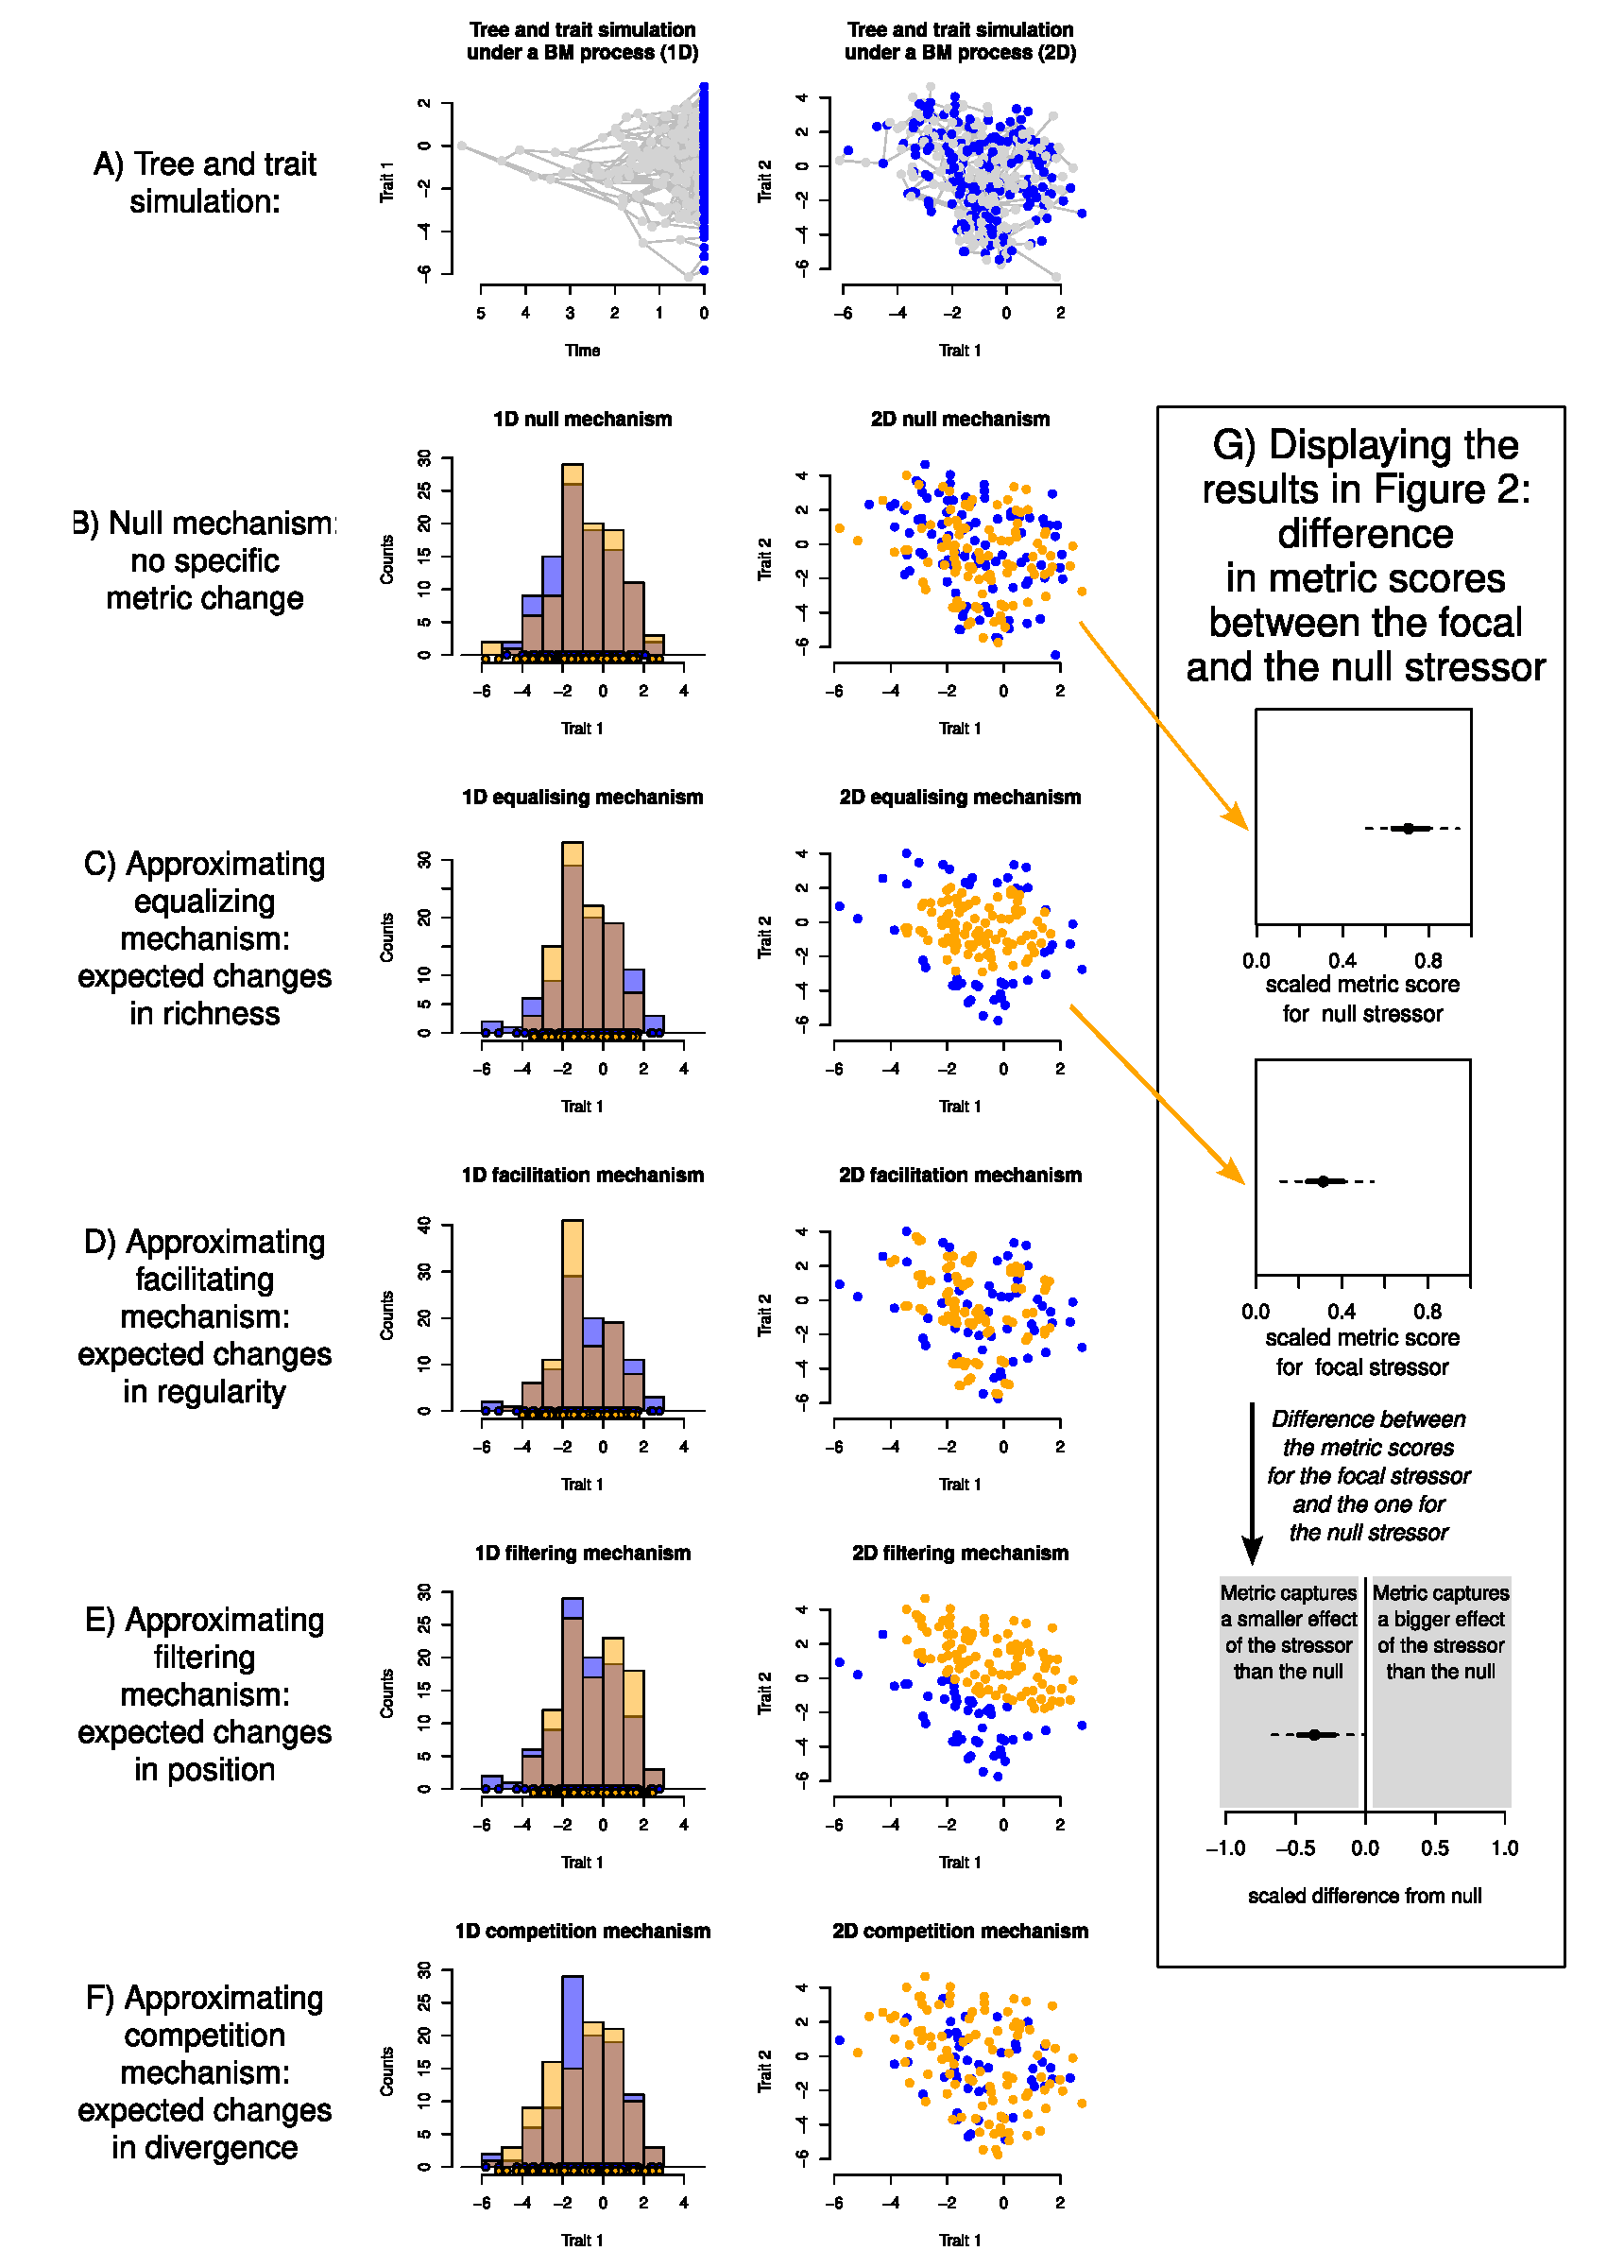
\includegraphics[width=0.5\textwidth]{Figures/simulation_protocol_explained.pdf}
\caption{\scriptsize{Illustration of the simulation protocol used in this paper.
A) we simulated a pure birth-tree with a trait evolving under a Brownian Motion process until reaching 200 observations resulting in a trait space of 2, 4, or 8 dimensions.
The first plot on row A illustrates one such simulation in one dimension through time (with time on the horizontal axis and trait value for one dimension on the vertical axis).
The second plot on the same row shows the same results but with a two dimensional trait represented here.
We then applied different stressors to the resulting trait space
We represent the elements removed by the stressors in blue and the ones kept in the trait space in orange.
The first column illustrate the distribution of the elements in one dimension with the overlap between the removed (blue) and kept (orange) elements in brown (note we did not measure any metric on 1D spaces)
The second column illustrate the same distributions in 2 dimensions.
We did not illustrate the distributions in 4 or 8 dimensions here.
We used the following stressors:
B) \textbf{null mechanism}: randomly removing a proportion of the observations;
C) \textbf{approximating equalising mechanism}: removing observations on the edge of the distribution;
D) \textbf{approximating facilitation mechanism}: removing observations to reduce the distance between pairs of observations (increasing local density; decreasing evenness);
E) \textbf{approximating filtering mechanism}: removing observations from one extreme of the distribution;
F) \textbf{approximating competition mechanism}: proportionally removing observations from the centre of the distribution.
The expected changes indicate the main type of metric affect by the stressor (following the aspects in \citealt{mammola2021concepts}).
G) we presented the results of the simulations as the scaled metric scores for the approximated mechanisms (C to F) relative to the null mechanism. The dot represents the median metric score and the thick and dashed lines respectively the 50\% and 95\% confidence intervals.}}
\label{Fig:simulations}
\end{figure}
\bigskip

\subsubsection{Metrics for measuring trait space occupancy (\textit{aka} functional diversity, dissimilarity, disparity):}

We structured our simulations based on three aspects of diversity commonly captured by functional diversity metrics (trait space occupancy metrics; \cite{mammola2021concepts}) using 12 metrics (Table \ref{Tab:metrics}):
1) Richness, encompassing metrics reflecting the sum of differences among observations; (4 metrics, equivalent to size metrics in \citealt{guillerme2020shifting});
2) Divergence, encompassing metrics reflecting the average differences among observations (4 metrics); and
3) Regularity, encompassing metrics reflecting how regular the differences among observations are (4 metrics, equivalent to density metrics in \citealt{guillerme2020shifting}).
Note that we focused here on three packages fully devoted to functional diversity analyses (\texttt{BAT} \citealt{cardoso2015bat} \texttt{FD} \citealt{Laliberte2010FD} and \texttt{TPD} \citealt{carmona2019trait}) in the \texttt{R} statistical environments (see \citealt{mammola2021concepts}).

\begin{table}
\center
\scriptsize
\begin{tabular}{p{0.1\linewidth}|p{0.15\linewidth}|p{0.15\linewidth}|p{0.2\linewidth}|p{0.15\linewidth}|p{0.1\linewidth}}

\textbf{Aspect} & \textbf{Method} & \textbf{Name} & \textbf{Description} & \textbf{\texttt{R} function} & \textbf{Reference}\\
\hline
Richness & Trait Probability Density & Functional richness & Sum of cells where trait probability density $> 0$ & \texttt{TPD::REND}* & \cite{carmona2019trait}\\
 & \cr 
 & Kernel density hypervolume & Functional richness & Size (volume) of the hypervolume & \texttt{BAT::kernel.alpha} & \cite{mammola2020functional}\\
 & \cr
 & Convex Hull & Functional richness & Volume of the convex hull & \texttt{BAT::hull.alpha} & \cite{cornwell2006trait}\\
 & \cr
 & Dendrogram & Alpha diversity & Total branch length of the functional dendrogram & \texttt{BAT::alpha} & \cite{petchey2002functional,cardoso2015bat}\\
\hline
Divergence & Trait Probability Density & Divergence & Overlap between the TPD function of a single observation and the TPD function of the whole set of observations & \texttt{TPD::REND}* & \cite{carmona2019trait}\\
 & \cr 
 & Kernel density hypervolume & Functional dispersion  & Average distance between an observation and a sample of random points within and the probabilistic hypervolume & \texttt{BAT::kernel.dispersion} & \cite{mammola2020functional}\\
 & \cr 
 & Dendrogram & Functional dispersion & Average dissimilarity between any two observations in the dendrogram & \texttt{BAT::dispersion} & \cite{cardoso2015bat}\\
 & \cr  
 & Distances & Rao's quadratic entropy & The mean Euclidean distance between every two random pairs of species & \texttt{FD::dbFD()\$RaoQ} & \cite{botta2005rao}\\
\hline
Regularity & Trait Probability Density & Functional evenness & An index of the spread of the trait distribution in an even spread of the distribution (e.g. the height of bins in a histogram) & \texttt{TPD::REND}* & \cite{carmona2019trait}\\
 & \cr 
 & Kernel density hypervolume & Functional evenness &  Overlap between a hypervolume and an imaginary hypervolume where dimensions are evenly distributed within their possible range & \texttt{BAT::kernel.evenness} & \cite{mammola2020functional}\\
 & \cr 
 & Dendrogram & Functional evenness & Regularity of abundances and distances between observations in the tree. & \texttt{BAT::evenness} & \cite{cardoso2015bat,cardoso2024calculating}\\
 & \cr 
 & Distances & Functional evenness & Regularity of abundances and distances along the minimum spanning tree linking all observations & \texttt{FD::dbFD()\$FEve} & \cite{Laliberte2010FD,villeger2008new}\\
\hline

\end{tabular}
\caption{\scriptsize{\textbf{Functional diversity metrics tested in our simulations.}}
}
\label{Tab:metrics}
* The \texttt{TPD} package currently only allows calculations for traitspaces up to four dimensions. This metric was exclude from traitspaces with more than four dimensions.
\end{table}

\subsubsection{Comparing and scaling the results to the random removals (null stressor)}

To understand the ability of each metric to capture a mechanism of interest, we compared their scores relative to the same metric scores of a null mechanism.
To ease interpretation of the results across a range of metrics with different orders of magnitudes of outputs and different random simulations, we first calculated the difference between the stressor of interest and the null stressor (e.g. $metric_{stressor20\%} - metric_{null20\%}$).
We then scaled these differences to be relative to the highest relative differences between all the simulations for that one metric and stressor (across the 4 levels of removal - 20\%, 40\%, etc.)
This resulted in each metric being scaled between $-1$ and $1$ where a negative difference can be interpreted as the random removal of elements leading to a higher metric score; a positive difference as the focal removal of elements (i.e. approximating equalisation, facilitation, filtering and competition) leading to a higher metric score; and a difference near $0$ meaning both the null stressor and the focal stressor having a similar effect on the metric score (Figs \ref{Fig:simulations}, \ref{Fig:simulation_results} and \ref{Fig:empirical_results}).
We interpret this last scenario as the metric score being unable to clearly distinguish between a random removal of elements and a non random one.
To assess these poor performances, we compared the distributions of the $171$ scores for each metric with each reduction level for each non-null stressor to the null stressor using pairwise t-tests.
The results of these tests are displayed in figure \ref{Fig:simulation_results} (for the non-null stressor, grey distributions are not clearly distinguishable from the null stressor).

\subsubsection{Measuring the effect of the strength of the stressor}

Finally, we measured the effect of the different strengths of the stressors (i.e. removing 20\%, 40\%, 60\% and 80\% the data) by fitting a linear regression using the scaled metric difference to the null score as a function of the amount of data removed
For each of these models, we reported the variance explained by the model (adjusted $R^2$) in the supplementary tables $2$ to $5$ and whether the slope was clearly distinguishable from $0$ (Figure \ref{Fig:simulation_results}; \textit{sensu} \citealt{dushoff2019can}).
This allowed us to see if there was any predictable linearity in the metric scores.
In other words testing whether the metric scores relative to null removals where linearly scaling with the amount of data removed.


\subsection{Empirical data}


We applied all metrics to an empirical dataset of bird extinctions on six Hawaiian islands (Hawaii, Kauai, Lanai, Maui, Molokai, Oahu), an archipelago which has suffered large numbers of anthropogenic extinctions due to a range of extinction drivers \citep{Walther2022}.
A prehistoric species list (avifauna known to be present prior to human colonisation of the islands), historic species list (avifauna known to be present at $1500$ CE) and extant species list of the native community for each island were taken from \cite{matthews2023global} along with trait values for the extinct species (\textit{Asio flammeus} was removed from the historic and extant species lists as its colonisation status is uncertain).
We also added two marine species to the prehistoric species list (\textit{Haliaeetus albicilla} and \textit{Pterodroma hypoleuca}); we compiled missing trait data for these two extinct species from \cite{sayol2021loss}.
We extracted traits for extant species from the AVONET database \citep{tobias2022avonet}.
We used $9$ morphological traits associated with dietary/foraging preference and dispersal ability \citep{pigot2020macroevolutionary,sheard2020ecological} to represent the functional diversity of the communities: mass; beak length (culmen); beak length (nares); beak width; beak depth; tarsus length; wing length; the length from the first secondary feather to the tip of the longest primary feather (Kipp's distance); and tail length.
Traits were log transformed and standardised to a mean of $0$ and standard deviation of $1$, prior to analyses.

The full trait dataset comprised $118$ bird species, all native species known to have existed on these islands over the last $125,000$ years.
$55$ species are known to have gone extinct prior to $1500$ CE and $26$ after $1500$ CE.
Note that we used the extinct species data as presented in \cite{matthews2023global}, and thus we do not include Hawaiian species declared extinct by the IUCN in $2024$.
For our analyses, we focused on two time periods: (i) the avifauna present in $1500$ CE (the ``historic dataset'') and (ii) the current native avifauna (``extant dataset'').
We represented the distinct reductions in species richness preceding these two time periods as our two stressors, the first one representing all pre-$1500$ CE extinctions (i.e., $118-55$ species; a species richness reduction of 46\%) and the second all the extinctions that have occurred until the present (i.e., $118-(55+26)$ species; a species richness reduction of 69\%).

To build the community trait space, we undertook a PCA including all $118$ species, which we then subset to calculate the trait space for the historic and extant datasets.
We selected the first $5$ axes to represent the trait spaces that explained at least 95\% of the variance in each specific group (historic and extant species - see supplementary figure 7; following the recommendations of \citealt{pigot2020macroevolutionary} and the dimensionality selection method from \citealt{guillerme2023innovation}).
We applied the same procedure as for the simulated data by simulating a null mechanism to compare to the observed ones by randomly removing $55$ and $81$ species for each stressor and scaling the results proportionally to this null mechanism (as described above).


\section{Results}

\begin{figure}[!htbp]
\centering
   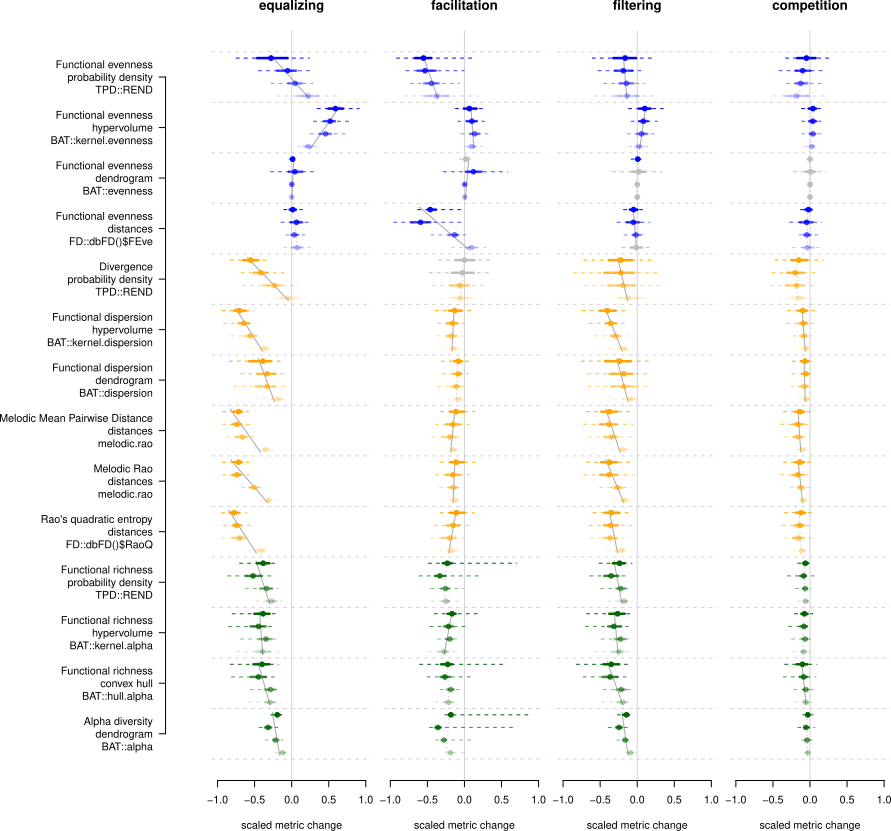
\includegraphics[width=0.8\textwidth]{Figures/results_per_metric_per_stressor_4d.pdf}
\caption{\scriptsize{\textbf{Simulation results:} the y axes represent the different metrics tested (sorted by categories).
The different columns represent the different stressors. The x-axes represent the metric values centred on the random changes and scaled by the maximum value for each metric between the four stressors.
Negative and positive values signify that the metric score for the stressor of interest is lower/higher than the one from the random stressor.
The dots represent the median metric value, the full line their 50\% confidence interval (CI) and the dashed line their 95\% CI.
The colours are here to visually separate the metrics by categories (green = richness, yellow = divergence, blue = regularity); the colour gradient within each row corresponds to a removal of respectively 80\%, 60\%, 40\% and 20\% of the data (from top to bottom).
The grey dots and corresponding CI lines represent distributions of metric scores not clearly distinguishable from the random metric scores (paired t-test $p$ value $> 0.05$).
Grey lines in the background across the distributions of different removal amounts represent the fitted linear model ``centred and scaled metric score function of the amount of data removed''.
Dashed thin grey lines represent non-significant linear models (slope's $p$ value $> 0.05$).
The model results (including $R^{2}$ and t-statistics) are available in supplementary table 3.
Similar figures are available in the supplementary materials for 2 and 8 dimensions.}}
\label{Fig:simulation_results}
\end{figure}
\bigskip

The ability of different metrics to capture the different patterns (and thus approximate the mechanisms) was highly variable.
It ranged from metrics capturing no clear pattern (e.g. the Functional evenness based on the dendrogram method for competition) to metrics clearly capturing one specific pattern (e.g. Divergence based on probability density for the equalising mechanism for a decrease in space occupancy).
Although most metrics captured a decrease in metric score relative to the amount of removed data, some metrics resulted in a score increase (e.g. the Functional evenness based on a hypervolume for the equalising mechanism) or non-linear responses (e.g. Alpha diversity based on a dendrogram for the equalising epresent distributions of metric scores; see supplementary tables 2 to 5 and 6 to 17).
Some cases resulted in an increase in metric score relative to random removals (positive values in Figure \ref{Fig:simulation_results}).
Furthermore, although we predicted some more common changes in aspects of functional diversity for some specific mechanisms, our simulations show that most metrics under most aspects (richness, divergence or regularity) capture changes of trait space occupancy under any mechanism (see caveats section in the discussion).

\begin{figure}[!htbp]
\centering
   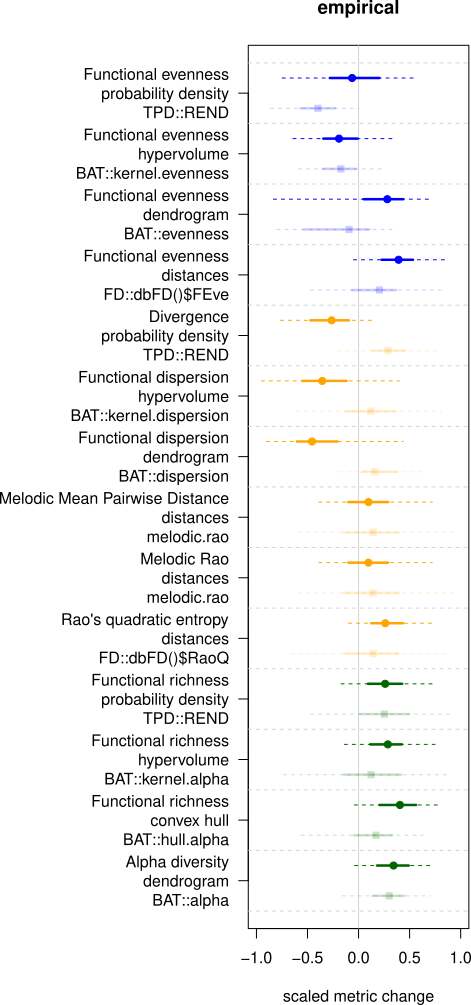
\includegraphics[width=0.4\textwidth]{Figures/results_per_metric_per_stressor_emp.pdf}
\caption{\scriptsize{\textbf{Empirical results:} the metrics and the scaled changes are measured in the same way as in figure 2 (green = richness, yellow = divergence, blue = regularity).
Plain circles represent the metrics for the species present on Hawaii at 1500 (historic data; 46\% removal - 63 species present) and fainted squares for the species currently present on Hawaii (extant data; 69\% removal - 37 species present).
The model results (including $R^{2}$ and t-statistics) are available in supplementary table 4.
}}
\label{Fig:empirical_results}
\end{figure}
\bigskip

For the empirical data, we see again a range of different possible interpretations depending on the metric describing the pattern (Figure \ref{Fig:empirical_results}, Supplementary table 5 and 18).
For example, all richness metrics (green; Figure \ref{Fig:empirical_results}) pick up a similar relative increase (i.e., relative to the null stressor) in richness for both the historic and extant datasets.
However, the results are occasionally contrasting between the historical and extant datasets, with a respective decrease and increase with some divergence metrics (e.g. functional dispersion based on dendrograms or hypervolumes).
Finally, some metrics pick up a decrease for both datasets (e.g. functional evenness based on hypervolumes - although the $95$\% confidence intervals overlapped with $0$).
Note that this apparent global increase in most metric values may appear counter intuitive given that $46$\% and $69$\% of species went extinct over the two time periods.
This is due to the scaling of the metrics compared to random equivalent extinctions.
That is, Figure \ref{Fig:empirical_results} is not displaying absolute changes in trait space occupancy but rather changes in trait space occupancy relative to a crude neutral model where all species are equally likely to go extinct.

\section{Discussion}

\subsection{Capturing approximated mechanisms with different metrics}

We tested 12 trait space occupancy metrics on simulated and empirical datasets to assess how each metric captures patterns of trait space changes based on stressors approximating ecological and evolutionary mechanisms.
Our results show that different metrics capture different patterns (what) leading to inferring different processes (how) that can be proposed to explain different mechanisms (why).
Therefore, the choice of trait space occupancy metric is essential to accurately describe a pattern of interest.
We found that different metrics can capture changes in pattern relative to the null mechanisms in different ways depending on the approximated mechanism of interest.
For example, for the approximated equalising mechanism, most metrics capture a pattern clearly smaller than the one from the null mechanism (i.e. randomly removing elements has more effects on the metric than removing them following the mechanism).
However, some metrics (e.g. the Functional evenness based on the hypervolume) capture a pattern clearly greater than the one from the null mechanism.
This means that changes in metric values can be counter intuitive and should always been interpreted in the context of the metric, data and question at hand.
Note also that, as mentioned above, different dimensionalities can have different effects on the metrics, depending on both the traitspace and the metric nature \citep{bellman1957dynamic}.

For example, say one is interested in looking at changes in functional diversity using a divergence metric calculated with the probability density method (e.g. \texttt{TPD::REND}).
They can apply this metric to their trait space and get two relative metric scores of $0.7$ and $0.65$ (pattern) for two levels of extinction (process).
The interpretation of this score as a change in functional diversity will depend on the worker's assumption of which mechanism affected the trait space.
In our simulations, if the mechanism approximated was the equalising one, the pattern can clearly be interpreted as a change in functional diversity, but if the mechanism is a facilitation one, the pattern can be meaningless (i.e. not clearly distinguishable from a null mechanism - Fig. \ref{Fig:simulation_results} shows this example by contrasting row 5, columns 1 and 2).
In this made up example, the procedure is done in reverse order where the the pattern is specified first and then the process and the mechanism (``What process and mechanism are needed to interpret pattern X?'').
In Box 2 we suggest an approach that specifies the process and the mechanism first (``how do I interpret pattern X under a specific process and mechanism''; see Box 2).

Regarding the different approximated mechanisms, it is interesting to note that our different approximations lead to different general behaviours of the metrics: for example the range of variance in the metric values is greater for the equalising mechanism and smaller for the competition mechanism (albeit nearly always distinguishable from the null mechanism).
These differences in metric variance across mechanisms suggest that some mechanisms lead to more subtle changes or/and that our approximation of these mechanisms can be variable (see caveats below).

\subsubsection{Empirical results}

The empirical results are also intriguing in that the loss of Hawaiian bird's functional diversity due to extinction is not greater than expected by chance (at least for certain metrics; Figure \ref{Fig:empirical_results}) because one would expect that extinctions target specific areas of functional diversity space (i.e. birds with specific trait combinations).
This contrasts with studies that have shown that species with certain traits (e.g., larger species) are more likely to have gone extinct and thus that functional diversity loss is larger than through random extinctions (e.g. \citealt{sayol2021loss,Matthews2022}).
This illustrates the importance of positing the mechanism and process of interest as well as the pattern to capture it before analysing the results.
For example, for the divergence metrics using probability density, hypervolume or dendrogram methods, we recovered changes in trait space that are smaller than expected by chance when focusing on all extinctions and larger than expected by chance when considering only pre-$1500$ extinctions.
This could lead to the interpretation that the trait space was not changed under any specific mechanism up to $1500$ (i.e. null mechanism) but that since then, specific mechanisms have been reducing specific areas of the trait space (e.g. filtering mechanism).
However, when using a different metric (say the Rao's quadratic entropy based on distance matrices), the results would indicate that a reduction of specific areas of the trait space could have also occured before $1500$ leading to very different interpretation of the results.


Our results show that the loss of  functional diversity for several metrics was not more than expected by chance.
This could be due to the taxonomic distribution of the extinct birds: this example data has approximatively $58$\% passerines while the majority of anthropogenic extinctions have been affecting non-passerines (approximatively $75$\%).
These species tend to be larger and possess more unique morphological traits (thus resulting in relatively large reductions in functional diversity).
However, in Hawaii, where the same proportion of known species were passerines (approx. $58$\%), the opposite is true: the majority of extinctions (approx. $60$\%) have been of passerine species.
It is important to note that we are not implying that there existed little morphological variation within extinct Hawaiian passerines - indeed, many of these extinctions involved the honeycreepers, a famous adaptive radiation involving substantial evolution of beak morphology \citep{Walther2022} - but simply that this morphological variation is less than that observed across all birds.
Given that the proportion of known Hawaiian species that are / were passerines roughly matches the proportion of extinct species that were passerines, our results indicate that these extinct species were more functionally similar than expected, thus relatively \textit{increasing} trait diversity (i.e. relative to random extinctions).
In addition, it is worth stressing that these analyses included marine species (which constitute less than 4\% of  known extinctions in Hawaii, while making up 11\% of the prehistoric assemblage) and different results may have been found if focusing exclusively on terrestrial birds.

More broadly, as can be seen from this empirical case, patterns are likely to be much less clear than with simulated data due to multiple stressors acting simultaneously.
For instance, extensive hunting is likely to present equalising and/or filtering pressure due to the selective hunting of larger bodied species.
In contrast, avian malaria, which is known to be an important extinction pressure of native Hawaiian birds \citep{samuel2011dynamics}, could show signals of a null mechanism since susceptibility to the disease is not trait-dependent (at least not in relation to the dimensions we have considered here), but is related to genetics (it mainly affects passerines, but there is considerable variation in susceptibility within passerines) and distributional range \citep{jessup2023wildlife}.

\subsection{Caveats}

Our results may be influenced by our choice of space occupancy metrics - specifically, we focused on metrics available in three statistical packages in \texttt{R}, the most common statistical language currently used in ecology \citep{lai2019evaluating}, but many others could have been used (e.g. \citealt{guillerme2020shifting}).
Also, our results are likely affected by the use of simplified stressors designed to approximate very complex ecological and evolutionary mechanisms by simply removing a percentage of observations in trait spaces in a non-random manner.
Note also that the simulated trait spaces here did not always share common characteristics with empirical trait spaces.
The simulated trait spaces in 2, 4 or 8 dimensions had the same variance on all dimensions (i.e. we used the same trait simulation process for all dimensions) whereas in empirical trait spaces, commonly generated using ordination techniques (e.g. PCA or PCO), the dimensions have by definition a decreasing variance.

Furthermore, we only presented results based on a relatively small number of dimensions (up to 8).
Although this number of dimensions is in the range of many studies in ecology (e.g. 6 dimensions in \citealt{healy2019animal}), it is not uncommon to use a much greater number of dimensions, especially in palaeontology (e.g. more than 200 dimensions in \citealt{van2023should}).
In a higher number of dimensions (usually $>$10 but this is highly variable depending on the system under study), metrics results are harder to scale linearly.
This sometimes makes metric interpretation more chaotic \cite{bellman1957dynamic} in the sense that there is no direct relationship between the number of observations and dimensions that can be used to extrapolate results in higher dimensional datasets.
In fact, the relationship between observations has an important effect on how our results scale with higher dimensionality (e.g. the volume of an evenly occupied space scales differently in high dimensions compared to the same space but with normally distributed observations).

Another cautionary note could be made about our choice of scaling the metrics relative to a random trait space reduction (with the same percentage of reduction).
This choice allowed us to simulate a null model designed to test whether the mechanisms of interest were causing the observed change in pattern \citep{bausman2018modeling}.
For example, if removing 80\% of the edges of a distribution was distinguishable or not from removing 80\% of a distribution randomly (e.g. facilitation mechanism measured as divergence using the probability density method - not distinguishable from null when removing 80\% or 60\% of the data; Figure \ref{Fig:simulation_results}).
Some metrics (e.g. Functional evenness using the dendrogram method) were not able to distinguish between the null mechanism and the mechanism of interest (here the mechanism simulating competition).
In other words, our statistical question was ``Does metric X distinguish between removing N\% of data in a biassed way (the mechanism) and removing N\% of data randomly (the null)?''.
This definition of null hypothesis is also appropriate for the empirical data if the question is the same.
However, it is very likely that researchers will ask a more exciting or intriguing question based on these data.
For example, an interesting one could be ``Are the extinctions spread uniformly in the trait space across all birds in Hawaii?".
This legitimate question would thus require first a trait space (the pattern - what) and maybe some contrasting groups of interest like extinctions through time (the process - how) to answer the question (the mechanism - why).
Furthermore, the scaling of the metrics paired with the levels of removal (80\%, 60\%, 40\% and 20\%) creates an expected artifact similarity when comparing the random removals against the other ones: when less data is available overall, the metrics are more likely to be similar (e.g. if removing 99\% of the data, we expect the random and removal metric score to be nearly identical to the non-random ones).

Importantly, it should always be borne in mind that mechanisms ought of course to be more complex in real world scenarios.
For example, evolutionary mechanisms can vary through time or across clades (and so patterns are often the results of multiple processes); and ecological mechanisms are often intertwined and work together to generate a pattern (e.g. facilitation + competition; \citealt{danet2024species}), or counteract each others by operating on the trait space in opposite directions (e.g., competition + filtering; \citealt{mammola2024functional})

\bigskip
\bigskip
\hrule
\hrule

\section*{Box 2: so which metric do \textit{I} choose?}

TL;DR: it depends!

Here is a proposed step by step protocol that could help one decide what to measure by clearly specifying their mechanism, process and pattern of interest prior to any functional diversity or disparity measurements.

\textit{We have data of bird traits for native species in Hawaii through time (e.g. before and after human colonisation of the archipelago).
We want to know how anthropogenic stresses (e.g. hunting, invasive species, land use change) have affected the trait diversity of native Hawaiian birds.}

\begin{figure}[!htbp]
\centering
   \includegraphics[width=0.5\textwidth]{Figures/empirical_example.pdf}
\caption{Example of a traitspace based on the empirical data described above.}
\label{Fig:trait_space_example}
\end{figure}
\bigskip

\subsubsection{Frame the question:}

\begin{itemize}

    \item \textbf{Why?} Think of the broad biological mechanism of interest. In our example, this could be asking why (due to what mechanism) has the community changed: \textit{the trait diversity has changed due to a filtering mechanism where anthropogenic stressors affect specific species with specific traits (e.g. through hunting, predation on eggs by mammals, etc...).}
    \item \textbf{How?} With the data we have at hand, identify the process we could analyse. In our example, this could be native bird species traits through time: \textit{how did filtering affect the native species after 1500?}

\end{itemize}

Although asking \textbf{why} and \textbf{how} is a relatively standard step in the literature, we suggest that proposing them in this framework more easily leads to the next, often less asked question of what pattern to capture:

\begin{itemize}
    \item \textbf{What?} Choose the appropriate pattern that would capture changes through time in relation to a filtering mechanism. In our example, this could be a continuous metric that measures either changes in the trait space position or/and changes in the trait space side. The idea being that filtering would remove either the edges or a specific portion of the trait space without affecting to many other parts of the trait space.
\end{itemize}


\subsubsection{Find the type of metrics of interest:}

Once the one has clearly defined the pattern they want to capture (\textbf{what}), we believe it gets easier to pick up the type of metric that would be the most adequate.
For example, we can follow the suggestions from \cite{mammola2021concepts} highlighting which kind of methodological pipeline best supports which type of metric of interest (Table \ref{Tab:box2}).

\begin{table}
\center
\begin{tabular}{c | c | c}
\textbf{Metric type}  & \textbf{Question} & \textbf{Are we interested?}\\
\hline
Size & Is one group bigger than another one? & Yes \\
Divergence & Is one group more spread than another one? & Not really \\
Regularity & Is one group more evenly disperse in space? & Not really \\
Something else  & Does the position of a group changes in space? & Yes \\
\end{tabular}
\caption{\textbf{Example of questions we can ask with the different metric types.}The categories are arbitrary and are taken from \cite{mammola2021concepts}}
\label{Tab:box2}
\end{table}


\subsubsection{Get the metric most appropriate to your data:}

So to describe the pattern for our specific example question, we will be interested in size and position of the trait space.
There is a lot of different metrics that capture changes in size and in position of the trait space and their choice should depend on the following questions:
Do you have a lot of data or not?
Do you have a lot of computational time available or not?
What type of data do you use (categorical, continuous, transformed)?
Are you familiar with the metric (is there a software implementation you can use)?
Of course, these are example questions and are not necessary the only ones you should ask.
\cite{mammola2021concepts} proposes a very handy flow chart.

Here following our experience and the nature of the data, we will measure the absolute size of the trait space using the convex hull size and the potential displacement of the trait space using the displacement metric \citep{guillerme2020shifting}.
Results are displayed in tables \ref{Tab:results_convhull} and \ref{Tab:displacement}.

\begin{table}[ht]
\centering
\begin{tabular}{lrr}
  \hline
 group & n & convex hull volume \\ 
  \hline
 current &  37 & 25.44 \\ 
 at 1500 &  63 & 60.84 \\ 
   \hline
\end{tabular}
\caption{Trait space size measured as the convex hull volume for both groups.}
\label{Tab:results_convhull}
\end{table}

\begin{table}[ht]
\centering
\begin{tabular}{lrrrrrr}
  \hline
 group & n & median displacement & 2.5\% & 25\% & 75\% & 97.5\% \\ 
  \hline
 current &  37 & 1.04 & 0.95 & 0.99 & 1.05 & 1.10 \\ 
 at 1500 &  63 & 1.12 & 0.85 & 0.94 & 1.19 & 1.34 \\ 
   \hline
\end{tabular}
\caption{Trait space position distribution measured as the displacement metric: the percentages are the confidence intervals of the distribution.}
\label{Tab:displacement}
\end{table}

Note that it is also possible to test whether the metric is actually capturing the broad mechanism of interest using evolutionary simulations (e.g. by simulating evolutionary scenarios that would include species traits that would go through a filtering mechanisms - \citealt{guillerme2024treats}) or, like in this manuscript, using stressors (e.g. by using the \texttt{moms} interactive package \citealt{guillerme2020shifting}).


\bigskip
\bigskip
\hrule
\hrule



\section{Conclusion}
Different ecological and evolutionary processes or mechanisms do not always results in different patterns.
Our results based on simulations and empirical data suggest that the same data can be interpreted differently depending on the choice of trait space occupancy metric (\textit{aka} disparity, dissimilarity or functional diversity metrics).
Different metrics are designed to capture different aspects \citep{guillerme2020shifting,mammola2021concepts} but also perform better or worse at their designed task depending on the data, the mechanism or/and process of interest.
Using space occupancy metrics for describing functional diversity is tricky.
This is because the metrics have properties that can be counter intuitive based on the data at hand.
And also because functions of ecosystems, or the organisms and niches within them, are hard to capture/understand/define.
This means that measuring functional diversity is based on both the definition of the metric and the function of interest and thus cannot be served by a one-fits-all metric.
In other words, it is important to choose a disparity/dissimilarity/functional diversity metric based on the question and the data at hand rather than as a default option or solely based on a previous inspiring publication.
We suggest caution when summarising patterns in observed data and propose a pipeline and tools for researchers to help understand how their pattern (often stemming from multidimensional data) can vary intuitively or not depending on the process and mechanism of interest.

\section{Repeatability and reproducibility}
The simulations, results figures and tables are entirely reproducible via \url{https://github.com/TGuillerme/eco_metrics_simulations}.
An additional vignette on how to choose metrics is available at \url{https://github.com/TGuillerme/eco_metrics_simulations/blob/master/Analysis/Choosing_metrics_vignette.Rmd}.


% \section{Acknowledgements}
% Thanks to Andrew Beckerman, Natalie Cooper, Alain Danet, Thomas Johnson and Gavin Thomas for comments on early versions of this manuscripts.
% TG was funded by the UKRI-NERC grant NE/X016781/1.
% SM was supported by NBFC, funded by the Italian Ministry of University and Research, PNRR, Missione 4, Componente 2, ``Dalla ricerca all'impresa'', Investimento 1.4, Project CN00000033.
% MWJ was supported by NERC CENTA2 grant NE/S007350/1 and University of Birmingham.



\bibliographystyle{sysbio}
\bibliography{references}


\end{document}
